\documentclass[11pt]{article}

% --- Essential Packages ---
\usepackage[utf8]{inputenc}
\usepackage[margin=1in]{geometry}
\usepackage{titlesec}
\usepackage{enumitem}
\usepackage{graphicx}
\usepackage{booktabs} 
\usepackage{amsmath}  
\usepackage{xcolor}
\usepackage{hyperref}

% --- Section Styling (Matching Style Guide) ---
\titleformat{\section}{\large\bfseries}{}{0em}{}[\titlerule]
\titleformat{\subsection}{\normalsize\bfseries\itshape}{}{0em}{}

% --- Header and Footer ---
\usepackage{fancyhdr}
\pagestyle{fancy}
\fancyhf{} % Clear all header and footer fields
\fancyhead[L]{CatNet}
\fancyhead[C]{Activity 1}
\fancyhead[R]{Spring 2026}
\renewcommand{\headrulewidth}{0.4pt} % Sets the line thickness

\hypersetup{
    pdfborder={0 0 0}
}

\begin{document}

\begin{center}
    \huge \textbf{Lab Activity: Surviving the Storm} \\
    \large \textit{PVST+ vs. Rapid PVST+ Convergence} \\
    \vspace{0.5em}
    \small \textbf{Module: CCNA Domain 2.0 - Network Access}
\end{center}

\vspace{1em}

\section{Scenario Overview}
You are a junior network engineer for a growing enterprise. Redundancy is critical: if a cable gets cut by a careless contractor, you need another path available so the business stays online. However, physically connecting switches in a loop creates a catastrophic problem: \textbf{Broadcast Storms}. 

\begin{figure}[ht]
    \centering
    % Left Image Block
    \begin{minipage}{0.48\textwidth}
        \centering
        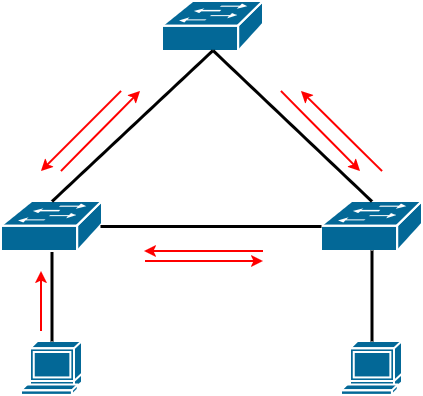
\includegraphics[width=\textwidth]{storm}
        \caption{Description of the storm}
        \label{fig:storm}
    \end{minipage}
    \hfill % This creates the space between the two images
    % Right Image Block
    \begin{minipage}{0.48\textwidth}
        \centering
        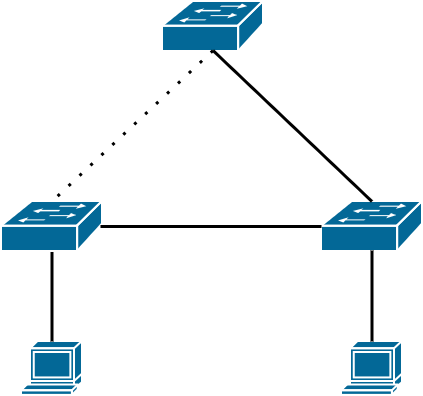
\includegraphics[width=\textwidth]{ST}
        \caption{Spanning Tree}
        \label{fig:st}
    \end{minipage}
\end{figure}

Without a loop-prevention mechanism, broadcast frames circulate endlessly, multiplying until the switches run out of memory and the network crashes. Your goal today is to wire a redundant network, observe a simulated outage, and tune the Spanning Tree Protocol (STP) to ensure the network recovers as fast as possible.

\section{Phase 1: Wiring \& Physical Setup}

Wire your three switches into a physical triangle (loop) and connect your PCs according to the topology diagram and addressing tables below.

\begin{center}
    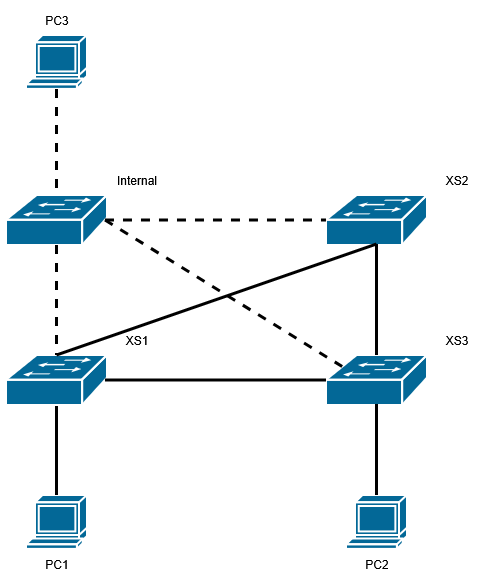
\includegraphics[width=0.5\textwidth]{diagram}
\end{center}

\vspace{0.5em}
\noindent\textbf{Host Addresses:}
\begin{center}
\resizebox{\textwidth}{!}{%
\begin{tabular}{@{}ccc|ccc@{}}
\toprule
\textbf{Desk} & \textbf{PC1 IP (/16)} & \textbf{PC2 IP (/16)} & \textbf{Desk} & \textbf{PC1 IP (/16)} & \textbf{PC2 IP (/16)} \\ \midrule
A & 10.12.50.101 & 10.12.50.201 & I & 10.12.50.109 & 10.12.50.209 \\
B & 10.12.50.102 & 10.12.50.202 & J & 10.12.50.110 & 10.12.50.210 \\
D & 10.12.50.104 & 10.12.50.204 & K & 10.12.50.111 & 10.12.50.211 \\
E & 10.12.50.105 & 10.12.50.205 & L & 10.12.50.112 & 10.12.50.212 \\
F & 10.12.50.106 & 10.12.50.206 & M & 10.12.50.113 & 10.12.50.213 \\
G & 10.12.50.107 & 10.12.50.207 & N & 10.12.50.114 & 10.12.50.214 \\ 
H & 10.12.50.108 & 10.12.50.208 & O & 10.12.50.115 & 10.12.50.215 \\ \bottomrule
\end{tabular}%
}
\end{center}

\vspace{0.5em}
\noindent\textbf{Switch Address:}
\begin{center}
\begin{tabular}{@{}cccc@{}}
\toprule
\textbf{Desk} & \textbf{Switch \#} & \textbf{ID Address} & Port \\ \midrule
A & 1 & 10.12.100.9 & 2003\\
A & 2 & 10.12.100.9 & 2004\\
B & 1 & 10.12.100.9 & 2011\\
B & 2 & 10.12.100.9 & 2012\\
D & 1 & 10.12.100.10 & 2003\\
D & 2 & 10.12.100.10 & 2004\\
E & 1 & 10.12.100.10 & 2011\\
E & 2 & 10.12.100.10 & 2012\\
F & 1 & 10.12.100.11 & 2003\\
F & 2 & 10.12.100.11 & 2004\\
G & 1 & 10.12.100.11 & 2011\\
G & 2 & 10.12.100.11 & 2012\\
H & 1 & 10.12.100.11 & 2019\\
H & 2 & 10.12.100.11 & 2020\\
\bottomrule
\end{tabular}
\quad
\begin{tabular}{@{}cccc@{}}
\toprule
\textbf{Desk} & \textbf{Switch \#} & \textbf{ID Address} & Port \\ \midrule
I & 1 & 10.12.100.12 & 2003\\
I & 2 & 10.12.100.12 & 2004\\
J & 1 & 10.12.100.12 & 2011\\
J & 2 & 10.12.100.12 & 2012\\
K & 1 & 10.12.100.13 & 2003\\
K & 2 & 10.12.100.13 & 2004\\
L & 1 & 10.12.100.13 & 2011\\
L & 2 & 10.12.100.13 & 2012\\
M & 1 & 10.12.100.13 & 2019\\
M & 2 & 10.12.100.13 & 2020\\
N & 1 & 10.12.100.14 & 2003\\
N & 2 & 10.12.100.14 & 2004\\
O & 1 & 10.12.100.14 & 2011\\
O & 2 & 10.12.100.14 & 2012\\
\bottomrule
\end{tabular}
\end{center}

\noindent\textbf{Linux PC Initialization (Run on PC1, PC2, and PC3):}
\begin{verbatim}
    sudo ip addr add <PC_IP>/16 dev eth0 broadcast +
    sudo ip link set dev eth0 up
\end{verbatim}

\vspace{0.5em}
\noindent \fbox{
    \parbox{0.95\textwidth}{
        \textbf{Stop \& Think:} Look at the LEDs on your switch ports connecting the switches together. You should see one port with an \textit{Amber/Orange} light. Why did the switch automatically block this specific port instead of the others? 
    }
}

\section{Phase 2: Baseline Benchmark (Legacy PVST+)}
By default, older Cisco switches might run standard IEEE 802.1D STP (or PVST+). Standard STP relies on static timers to ensure a loop-free topology before forwarding traffic.

\[
\text{Link Down} \rightarrow \text{Listening (15s)} \rightarrow \text{Learning (15s)} \rightarrow \text{Forwarding}
\]

\noindent\fbox{
    \parbox{0.96\textwidth}{
        \textbf{Access Note:} If prompted for a password to enter privileged mode, use: \texttt{chico}
    }
}

\vspace{1em}
\noindent\textbf{Verify Current State (Run on all switches):}
\begin{verbatim}
    XS1> enable
    XS1# configure terminal
    XS1(config)# spanning-tree mode pvst
    XS1(config)# end
    XS1# write memory
    XS1# show spanning-tree
\end{verbatim}
\textit{Note the "Root ID" and "Bridge ID" MAC addresses. Is this switch the Root Bridge?}

\subsection*{Test 1: The 50-Second Blackout}
Let's simulate a cable cut. We will run a continuous ping that explicitly flags dropped packets using the \texttt{-O} flag.

\noindent On PC1, begin the ping test to PC2:
\begin{verbatim}
    ping -O -c 100 <PC2_IP>
\end{verbatim}
\textbf{Action:} While the ping is running, unplug one of the \textit{active} switch-to-switch cables (green LEDs on both sides). \\
\textbf{Observation:} Count the number of dropped packets. Each drop represents roughly one second of network downtime. You should expect around 30 to 50 seconds of complete blackout before the amber light turns green.

\section{Phase 3: The Upgrade (Rapid PVST+)}
In a modern enterprise, 30 seconds of downtime drops VoIP calls, disconnects databases, and halts production. Rapid Spanning Tree Protocol (IEEE 802.1w) fixes this by replacing passive timers with an active negotiation handshake.

\noindent\textbf{Configure RPVST+ (Run on all 3 switches):}
\begin{verbatim}
    XS1# clear spanning-tree detected-protocols
    XS1# configure terminal
    XS1(config)# spanning-tree mode rapid-pvst
    XS1(config)# end
    XS1# write memory
    XS1# show spanning-tree
\end{verbatim}

\subsection*{Test 2: The 2-Second Hiccup}
Reconnect the severed link and wait 30 seconds for the network to stabilize. 
Run the ping command from PC1 again: \texttt{ping -O -c 100 <PC2\_IP>}. \\
\textbf{Action:} Unplug the active link again. \\
\textbf{Observation:} Compare the packet loss to Test 1.

\vspace{0.5em}
\noindent \fbox{
    \parbox{0.95\textwidth}{
        \textbf{Stop \& Think:} The downtime was drastically reduced, but was it zero? RPVST+ is fast, but it still requires the switches to process the topology change. How could we design the network to have literally zero packet loss? (Hint: Think about link aggregation or routing protocols).
    }
}

\section{Phase 4: Network Engineering (Tuning the Tree)}
By default, switches elect the Root Bridge based on the lowest MAC address. This means your oldest, slowest switch might accidentally become the core of your network. \textbf{We must dictate the topology manually.}

\vspace{1em}
Additionally, ports connected to PCs don't create loops. We can use \texttt{portfast} to tell the switch to skip the STP handshake entirely on edge ports, bringing them up instantly.

\noindent\textbf{1. Force Switch 1 to be the Primary Root:}
\begin{verbatim}
    XS1(config)# spanning-tree vlan 1 priority 4096 
\end{verbatim}

\noindent\textbf{2. Force Switch 2 to be the Secondary Failover:}
\begin{verbatim}
    XS2(config)# spanning-tree vlan 1 priority 8192
\end{verbatim}

\noindent\textbf{3. Enable PortFast on PC Connections (Do on all PC-facing ports):}
\begin{verbatim}
    XS1(config)# show ip interface brief  <-- [TODO: Explain command]
    XS1(config)# interface FastEthernet 0/1/0  <-- Use your specific port
    XS1(config-if)# spanning-tree portfast
\end{verbatim}
\textcolor{red}{\textbf{WARNING:}} Never plug a switch into a PortFast-enabled port. 

\vspace{0.5em}
\noindent \fbox{
    \parbox{0.95\textwidth}{
        \textbf{Stop \& Think:} Discuss why we should not plug a switch into a PortFast-enabled port.
    }
}

\subsection*{Test 3: The Optimized Network}
Reconnect all cables. Wait for stability. Run your ping test one final time and cut the active link. Because you have optimized the Root Bridge location and edge ports, your failover should be incredibly efficient.

\vspace{1em}
\noindent\textbf{Bonus Automation Challenge:} 
In the CCNA exam, you must understand network programmability. Write a bash shell script to Telnet into all three switches and apply the \texttt{rapid-pvst} and \texttt{portfast} configurations automatically. The hints are available at \url{https://github.com/CatNetChico/activity-1}. 

\newpage

\section*{Appendix: Resume Building}
\addcontentsline{toc}{section}{Appendix: Resume Building}

\textit{After completing this lab, you have gained practical, hands-on experience with Layer 2 redundancy and convergence optimization. You can adapt the following bullet points for your resume to accurately highlight the skills you demonstrated today:}

\vspace{0.5em}
\noindent \textbf{Relevant Experience / Academic Projects:}
\begin{itemize}[leftmargin=*, itemsep=2pt]
    \item \textbf{Layer 2 Infrastructure Optimization:} Migrated legacy Spanning Tree topologies to \textbf{IEEE 802.1w (RSTP)}, reducing link-failure convergence time from 50 seconds to sub-2-second intervals.
    \item \textbf{Network Stability \& High Availability:} Engineered deterministic Layer 2 traffic flows by manually calculating and assigning \textbf{Root Bridge} and Secondary Root Bridge priorities.
    \item \textbf{Edge Port Tuning:} Deployed \textbf{PortFast} on edge access ports to eliminate DHCP timeout issues and transition delays while preventing \textbf{Broadcast Storms}.
    \item \textbf{Disaster Simulation \& Benchmarking:} Utilized continuous ICMP packet analysis to quantify network downtime and validate failover mechanisms during physical hardware loss.
\end{itemize}

\vspace{1em}
\noindent \textbf{Core Skills Acquired:} Layer 2 Switching, Spanning Tree Protocol (STP/RSTP), High Availability Design, Network Benchmarking, Cisco IOS Configuration.

\end{document}